\problemname{Astronomer}
\illustration{.3}{img/TychoBrahe.JPG}{}

\noindent
% The astronomer has a passion for stargazing.
% In particular, he gets immense pleasure out of gazing at $k$~stars simultaneously through his telescope.
% Building a telescope with radius~$r$ costs $t\cdot r$~kroner.
% A newly built telescope will point exactly at the origin $(0,0)$.
% Moving it to point somewhere else also takes effort;
% shifting the telescope a distance of $d$~units incurs a cost of $s\cdot d$~kroner.
% The astronomer can observe all stars at distance at most $r$ from where the telescope points.
Астроном має пристрасть до спостереження за зірками.
Зокрема, він отримує незміренне задоволення від спостереження за $k$ зірками одночасно через свій телескоп.
Побудова телескопа з радіусом $r$ коштує $t\cdot r$ гривень.
Новозбудований телескоп буде спрямований точно на початок координат $(0,0)$.
Переміщення телескопа в іншу точку також вимагає зусиль;
пересування телескопа на відстань $d$ одиниць коштує $s\cdot d$ гривень.
Астроном може спостерігати всі зірки на відстані, не більшій за $r$ від місця, на яке спрямований телескоп.

% How much does it cost to build and move a telescope that allows $k$~stars to be observed at once?
Скільки коштує побудова та переміщення телескопа, який дозволяє спостерігати одночасно $k$ зірок?

\medskip

% All coordinates and distances are given in the Euclidean plane.
Усі координати та відстані задані в Євклідовій площині.


\section*{Приклад}

% Here is an example with $n=3$ stars at positions $(0,0)$, $(2,0)$, and $(3,1)$.
% The shaded area shows a telescope of radius~$1$ pointing at $(1,0)$ covering two stars; this costs $s + t$~kroner and is an optimal solution to sample input~$3$.
% The image also shows optimal solutions to sample inputs~$1$, $2$, and $4$.
Ось приклад з $n=3$ зірками на позиціях $(0,0)$, $(2,0)$ та $(3,1)$.
Заштрихована область показує телескоп з радіусом $1$, спрямований на $(1,0)$, який охоплює дві зірки; це коштує $s + t$ гривень та є оптимальним рішенням для вхідних даних з прикладу~$3$.
Зображення також показує оптимальні рішення для прикладів з вхідними даними $1$, $2$ та $4$.

\medskip
\noindent
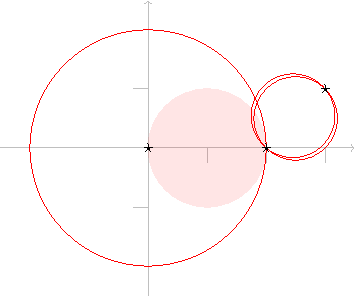
\includegraphics[width=.3\textwidth]{img/samples.pdf}


% \section*{Input}
\section*{Вхідні дані}

% The first line consists of four integers:
% the number~$k$ of stars the astronomer wants to observe,
% the number~$n$ of stars in tonight's sky,
% the shifting cost~$s$, and
% the telescope building cost~$t$.
% Then follow $n$ lines, where the $i$th line contains the integer coordinates $x_i$ and $y_i$ of the $i$th star.
Перший рядок містить чотири цілих числа:
кількість $k$ зірок, які астроном хоче спостерігати,
кількість $n$ зірок на сьогоднішньому небі,
вартість переміщення $s$ та
вартість побудови телескопа $t$.
Потім слідують $n$ рядків, де $i$-й рядок містить цілочисельні координати $x_i$ та $y_i$ $i$-ї зірки.

% \section*{Output}
\section*{Вихідні дані}

% A single real number: the minimum number of kroner that the astronomer needs to spend.
Одне дійсне число: мінімальна сума грошей, яку астроном повинен витратити.

% \section*{Constraints and Scoring}
\section*{Обмеження та оцінювання}

% You can assume
Ви можете припускати, що
\begin{enumerate}
\item $1\leq k\leq n\leq 700$. % constraint:kn
\item $x_i, y_i\in \{-10^9,\ldots, 10^9\}$ для всіх $i\in\{1,\ldots,n\}$. % constraint:xy
\item $s,t\in \{0,\ldots, 10^9\}$. % constraint:st
% \item Your output is accepted if it is within a relative or absolute tolerance of $\epsilon = 10^{-6}$ of the correct answer.
\item Ваш вивід буде прийнятий, якщо він знаходиться в межах відносної або абсолютної точності $\epsilon = 10^{-6}$ від правильної відповіді.
\end{enumerate}


% Your solution will be tested on a set of test groups, each worth a number of points.
% Each test group contains a set of test cases.
% To get the points for a test group you need to solve all test cases in the test group.
% Your final score will be the maximum score of a single submission.
Ваше рішення буде перевірятися на наборі тестових груп, кожна з яких оцінюється певною кількістю балів.
Кожна тестова група містить набір тестових випадків.
Щоб отримати бали за тестову групу, вам потрібно вирішити всі тестові випадки в цій групі.
Остаточний бал буде максимальним балом за одну спробу.

\medskip
\noindent
\begin{tabular}{lll}
%  Group & Points & Constraints\\\hline
  Група & Бали & Обмеження\\\hline
  $1$ & $18$ &  $t\leq s$\\
  $2$ & $17$ & $n\le 50$ and $s=0$\\
  $3$ & $15$ & $s=0$\\
  $4$ & $12$ & $n\leq 50$\\
  $5$ & $14$ & $n\leq 350$\\
  $6$ & $10$ & $\epsilon = 1/10$\\
%  $7$ & $23$ & \emph{No further constraints}\\
  $7$ & $14$ & \emph{Немає додаткових обмежень}\\
\end{tabular}



